Este capítulo tem como objetivo apresentar uma base teórica de todos os conceitos necessários para o entendimento das demais seções deste trabalho. Primeiramente, será explorado o que é aprendizagem de máquina e algumas classificações úteis. Subsequentemente, será explicado os conceitos básicos por trás de cada um dos modelos utilizados nesse trabalho. Para a explicação de alguns modelos, será necessária uma elucidação prévia de alguns conceitos fundamentais por trás de seu funcionamento. Ou seja, será explicado o conceito de árvores de regressão para depois ser explicado o funcionamento de \textit{\acrshort{RF}} e, posteriormente, será explicado o que é uma \textit{\acrshort{RNN}}, para que seja possível explicar como funcionam os modelos \textit{\acrshort{LSTM}} e \textit{\acrshort{GRU}}.

\section{Aprendizagem de Máquina}

No livro \textit{Machine Learning: a Probabilistic Perspective} \cite{murphy2012machine}, aprendizagem de máquina é definida como um conjunto de técnicas que encontram, automaticamente, padrões em um dado conjunto de dados, que pode estar imperfeito ou incompleto para determinado problema. Também é dito que a aprendizagem de máquina utiliza os padrões descobertos para tentar prever ou decidir algo. Para realizar tal tarefa, existe uma variedade de técnicas, mas que são sempre classificadas como supervisionadas, não-supervisionadas, ou de reforço. A classificação se dá pela maneira como o algoritmo utilizado aprende o padrão dos dados.

Técnicas não-supervisionadas são aquelas que buscam, a partir de um conjunto de dados(\(\set{x_i \mid 1\leq i\leq N}\)) utilizado como entrada do algoritmo, prever sua a saída, mas sem nenhum tipo de comentário sobre suas previsões e/ou classificações. Ou seja, a aprendizagem é feita sem que se conheça o formato da saída ideal do algoritmo. Esse tipo de técnica é utilizada em problemas menos definidos no que diz respeito ao tipo de saída esperada. Técnicas de reforço são aquelas que tentam aprender a partir da tentativa e erro, dado que o problema forneça recompensa e/ou punição para certas ações. Esse tipo de técnica pode ser usada para ensinar um robô a jogar \textit{Tetris}, por exemplo.

Técnicas supervisionadas são aquelas que tentam mapear uma entrada a uma saída correspondente (\(f(x) = y\)). Normalmente, essas técnicas utilizam de um conjunto de pares de entrada e saída (\(\set{(x_i, y_i) \mid 1\leq i\leq N}\)) para aprender a fazer o mapeamento, isto é, utilizam um conjunto de treinamento para aprender, onde o treinamento é testado sobre um conjunto de teste, ou seja, existe um \textit{feedback} quanto a previsão do algoritmo. Por exemplo, a entrada de um determinado algoritmo poderia ser uma imagem ou um conjunto de características de um medicamento. Caso a saída seja do tipo nominal, a técnica é do sub-tipo classificador. Caso a saída seja do tipo ordinal, a técnica é do sub-tipo regressor.

\subsection{Paramétrico e Não-paramétrico}

As técnicas de aprendizagem de máquina também podem ser classificadas de acordo com as suposições feitas por elas sobre o conjunto de dados utilizados. Essas classificações podem ser paramétricas ou não-paramétricas. Técnicas paramétricas dispõe de um número fixo de parâmetros para tentar descrever os dados, supondo assim que os dados seguem uma distribuição específica. Um exemplo de modelo paramétrico seria a regressão linear, que utiliza uma equação com parâmetros fixos para traçar uma reta que melhor representa a distribuição dos dados. Já modelos não-paramétricos possuem um número variável de parâmetros que dependem dos dados utilizados. Desse modo, não é feita uma suposição de que existe uma distribuição específica nos dados. Modelos paramétricos levam a vantagem na questão de velocidade de treinamento, porém perdem na questão flexibilidade. A escolha de qual tipo utilizar depende muito do formato dos dados do problema e do seu tamanho, dentre outros fatores.

\section{Árvores de Regressão}

De acordo com Trevor Hastie et. al. no Livro \textit{The Elements of Statistical Learning}, árvore é uma técnica que pode ser utilizado para aprendizagem de máquina supervisionada. No qual pode ser usado tanto para classificação (árvores de decisão), quanto para regressão (árvores de regressão). Elas são consideradas extremamente poderosas e simples de entender. Basicamente, árvores dividem o espaço de características utilizando de regras.

Árvores utilizam de um algoritmo guloso. Isto é, os melhores resultados locais fazem parte do melhor resultado global. Inicialmente, o algoritmo escolhe uma das características e define uma regra a partir da mesma. Assim, dividindo os dados em dois conjuntos. Por exemplo, considere que uma característica seja idade, uma regra possível seria \texttt{Idade \(\leq\) 40}. Seguindo esta regra o algoritmo divide os dados. Para os conjuntos resultantes, é definido uma nova regra e isso acontece sucessivamente até que não seja mais possível dividir os dados.

Existem algumas formas de decidir qual o melhor par, característica e regra, para um conjunto de dados. Uma das formas possíveis seria: para cada uma das características, ou conjunto de características, determina-se a melhor regra que divide o conjunto de dados no nó atual e compara essas regras para determinar qual o melhor par. Desta forma, é possível comparar os pares resultantes com um custo aceitável. A comparação entre os pares pode ser feita de diversas formas, para classificação pode ser usado o \textit{Gini Index} e para regressão pode ser usado a Soma do Erros Quadráticos. Uma vez construída a árvore, para utilizá-la basta percorrê-la seguindo as regras já definidas, assim como mostrado na Figura \ref{figure:tree}.

É importante notar a grande flexibilidade desse modelo de se ajustar ao conjunto de dados, isto é, árvores podem sofrer com o problema do sobre-ajuste (\textit{overfitting}). Por exemplo, é possível que o modelo tenha em cada folha da árvore um elemento do conjunto de dados. Para resolver este problema, é necessário controlar certos aspectos da construção da árvore, como a sua altura máxima, ou o limite mínimo de tamanho necessário para se dividir o conjunto. O autor sugere utilizar o segundo método, seguido de uma redução da árvore resultante, porém, dependendo dos dados, podem vir a existir modelos de construção melhores.
 
 \begin{figure}[htbp]
    \centering
    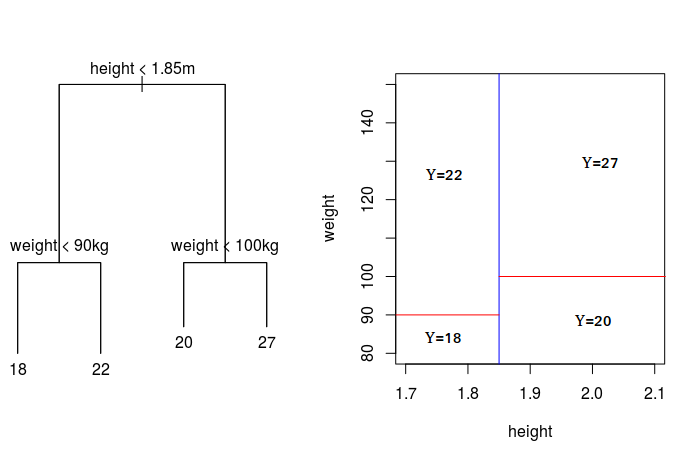
\includegraphics[scale=0.6]{monography/img/models/regression_tree.png}
    \label{figure:tree}
    \caption[Árvore de Regressão Dividindo o Espaço de Resposta]{Árvore de Regressão Dividindo o Espaço de Resposta\footnotemark}
\end{figure}

\footnotetext{\url{https://www.r-bloggers.com/how-random-forests-improve-simple-regression-trees/}}

\section{\acrfull{RF}}

Criado por Leo Breiman em \textit{Random Forest} \cite{Breiman:2001:RF:570181.570182}, \textit{\acrshort{RF}} é um método de aprendizagem de máquina utilizado tanto para classificação quanto para regressão. Segundo o autor, o método é uma combinação de árvores, de decisões ou regressão, onde cada árvore depende de uma amostra aleatória, sendo esta amostra independente do conjunto de dados. Além disso, todas as árvores devem possuir a mesma distribuição. 

A construção das árvores é feita utilizando o método \textit{Bagging} (\textit{\textbf{B}ootstrap \textbf{Agg}regation}), também criado por Leo Breiman em \textit{Bagging Predictors} \cite{Breiman:1996:BP:231986.231989}. Este método gera várias versões de um mesmo modelo e agrega os resultados dos mesmos. As versões do modelo utilizam amostras do conjunto de dados selecionadas aleatoriamente, mas com a mesma distribuição.

Porém, diferente de \textit{Bagging}, \textit{\acrshort{RF}} utiliza mais uma técnica para diminuir o sobre-ajuste (\textit{overfitting}). Há uma modificação no algoritmo de criação das árvores de decisão limitando a quantidade de características (\textit{features}) do conjunto de dados que vai ser utilizada. O autor sugere limitar a quantidade de características (\textit{q}) para $ \sqrt{q} $, no caso de classificação, ou $ \frac{q}{3} $, no caso de regressão \cite{hastie2005elements}. Além disso, o autor também sugere, no artigo original, que, para selecionar a quantidade ideal de características deve-se utilizar de estimativas \textit{out-of-bag}, explicadas também no artigo.

Como \textit{\acrshort{RF}} é uma combinação de outros modelos de aprendizagem de máquina, ela pode ser classificada como um Comitê de Máquinas (\textit{Ensemble Learning}). A forma como as respostas de cada uma das máquinas são combinadas depende do problema. Para classificação pode ser usado uma votação (voto da maioria) e para um problema de regressão pode ser usado uma média dos valores, assim como mostrado na Figura \ref{figure:random_forest}.

\begin{figure}[htbp]
    \centering
    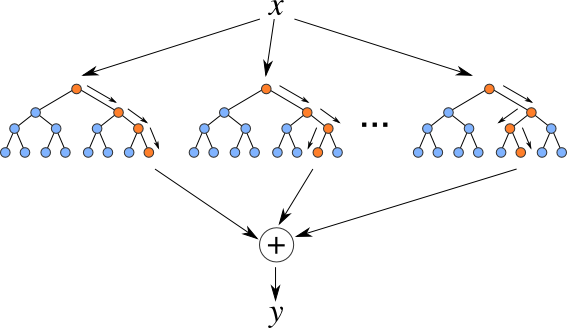
\includegraphics[scale=1.0]{monography/img/models/random_forest.png}
    \label{figure:random_forest}
    \caption[Representação do funcionamento de uma \textit{\acrshort{RF}}]{Representação do funcionamento de uma \textit{\acrshort{RF}}\footnotemark}
\end{figure}

\footnotetext{\url{https://dsc-spidal.github.io/harp/img/4-5-1.png}}

\section{\acrfull{SVM}}

\textit{\acrshort{SVM}} foi criado originalmente por Vladimir Vapnik nos anos 60 e foi evoluindo até se tornar o que é hoje  \cite{Smola03atutorial}. Essa técnica é não-paramétrica e supervisionada, sendo que a ideia básica por trás pode ser usada tanto para classificação quanto para regressão.

% TODO: falar de onde o nome veio (o que são os support vector machines)

% TODO: falar como ela é e da insensibilidade epsilon
%No caso da regressão, tenta-se criar uma função \(f(x)\) de forma que se \(g(x)\) é a função que perfeitamente descreve o conjunto de dados e \(\epsilon\) seja a dimensão do erro, para todo \(f(x)\)  \(\abs{g(x) - f(x)} \leq \epsilon \).

% TODO: falar sobre as caracteristicas iterativas
%A aprendizagem do modelo é iterativa.

% TODO: falar do mapeamento para outra dimensão pode auxiliar na SVM
%Só que nem todo o problema pode ser resolvido com qualquer coisa, porem pode ser resolvido em outra dimensão.

Mapear todo um conjunto de dados para outra representação do espaço é computacionalmente intenso. Porém uma função \textit{Kernel} consegue mapear dois pontos que pertencem a algum certo espaço para a distância deles em alguma outra representação desse espaço. Esse mapeamento é menos exigente computacionalmente, tornando então desnecessário mapear todo o conjunto de dados para a outra representação. Porém, mesmo com o \textit{Kernels}, \textit{\acrshort{SVM}} não escala muito bem para conjunto de dados muito grandes \cite{chollet2018deep}.

% TODO: just mention that you can do this and on methodology you say the variable that does it
Para ajustar a \textit{\acrshort{SVR}} podemos controlar o tamanho do tubo (\(\epsilon\)) e, entre outros, quão influentes são os pontos que não localizados no tubo (C). A variável C dessa técnica indica quanto os erros serão penalizados. Se for baixo, erros não serão muito penalizados e se for alto os erros serão muito penalizados. Além disso, alguns \textit{Kernels} possuem variáveis (\(\gamma\)), por exemplo) que ajudam no ajuste da função aos dados. \(\gamma\) determina a influência dos \textit{support vectors} no treinamento. Quanto maior o valor, menor a influência do \textit{support vectors}, quanto menor o valor, maior a influência. Valores baixos podem levar a uma função que não se ajusta muito ao conjunto de dados, prono a sub-ajuste. Já valores altos podem levar a uma função que se ajusta muito ao conjunto de dados, prono a sobre-ajuste.

% TODO: Mostrar exemplo simples de 1 dimensão




\begin{figure}[htbp]
    \centering
    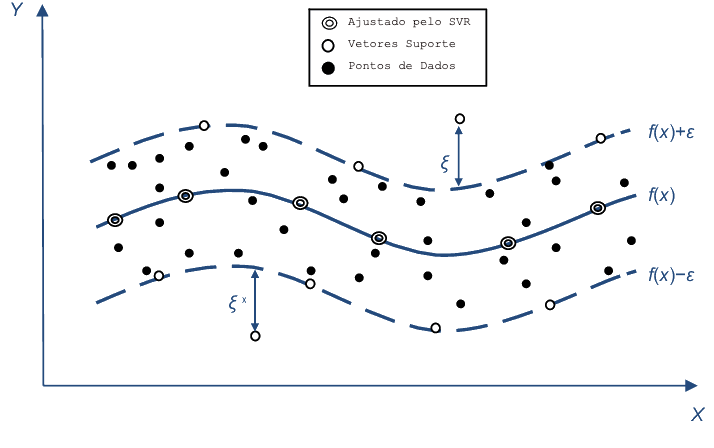
\includegraphics[scale=1.0]{monography/img/models/svr_example.png}
    \label{figure:support_vector_machine}
    \caption[Representação do funcionamento de uma \textit{\acrshort{SVM}}]{Representação do funcionamento de uma \textit{\acrshort{SVM}}\footnotemark}
\end{figure}

\footnotetext{\url{https://www.researchgate.net/figure/Schematic-of-the-one-dimensional-support-vector-regression-SVR-model-Only-the-points_fig5_320916953}}


\section{\acrfull{RNN}}
% RESOURCE: to explain recurrent neural networks (http://d2l.ai/chapter_recurrent-neural-networks/index.html)

% TODO: adiconar referência de onde vc tirou essa explicação

% TODO: Falar que sofre de memória curta e outros defeitos

% TODO: veja esse coisa apra explicar melhor LSTM e RNN (https://www.youtube.com/watch?v=6niqTuYFZLQ)

\textit{\acrshort{RNN}} surgiu da incapacidade de redes neurais comuns (\textit{\acrshort{NN}}) de levar em consideração resultados produzidos anteriormente pela rede. Resultados esses que poderiam vir a influenciar o resultado atual. Ou seja, redes neurais artificiais comuns, ou do tipo \textit{feedforward} utilizam apenas do seu estado atual para gerar sua saída. Para exemplificar, considere um problema de classificação, onde, a partir de uma imagem de um cachorro, ou gato, uma rede neural deva ser capaz de dizer corretamente qual animal a imagem representa. Para cada rodada de classificação, a imagem utilizada na rodada passada não importa, pois uma não tem relação direta com a outra. 

Porém, existem determinados problemas que exigem certa correlação entre os dados, como por exemplo, interpretar um documento, entender o contexto de um filme, ou avaliar a oscilação de uma bolsa de valores ao longo do tempo. Como descrito por Mitchell em \textit{Machine Learning} \cite{Mitchell_1997}, \textit{\acrshort{RNN}} são mais adequadas para estas situações, pois nesse tipo de problema, dados isolados não tem tanto significado quanto o conjunto, o que exige um conceito de memória. Para simular este efeito de memória, \textit{\acrshort{RNN}} dispõe de uma arquitetura onde a saída do nó anterior é utilizada como entrada no nó seguinte, juntamente com a entrada nova atual da rede. Para passar estes valores de um nó para o outro, a \textit{\acrshort{RNN}} dispõe de um mecanismo chamado \textit{Hidden Layer}. Na Figura \ref{figure:rnn} é exemplificada a sua arquitetura, onde o último resultado utiliza como entrada valores resultantes das execuções anteriores.

\begin{figure}[htbp]
    \centering
    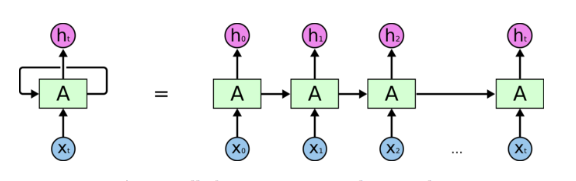
\includegraphics[scale=0.4]{monography/img/models/rnnExample.png}
    \label{figure:rnn}
    \caption[Representação simples do conceito de um RNN]{Representação simples do conceito de uma RNN \footnotemark}
\end{figure}

\subsection{\acrfull{LSTM}}

% TODO: cite a book

\textit{\acrshort{LSTM}} é um método proposto pela primeira vez por Sepp Hochreiter e Jurgen Schmidhuber em \textit{Long short-term memory} \cite{doi:10.1162/neco.1997.9.8.1735}. Ele é utilizado para predição de informações que derivam de dados sequenciais e séries temporais, sendo possível encontrar diversos trabalhos na literatura que mostram sua eficiência quando comparado a outros métodos. \acrshort{LSTM} é um tipo de \acrshort{RNN} que utiliza de estados anteriores e do estado atual da rede para gerar sua saída \cite{Xiaolei_2015, Zainab_2018}. Ao utilizar dos estados anteriores, a \acrshort{RNN} acaba por simular uma memória, melhorando sua capacidade de aprender. 

\begin{figure}[htbp]
    \centering
    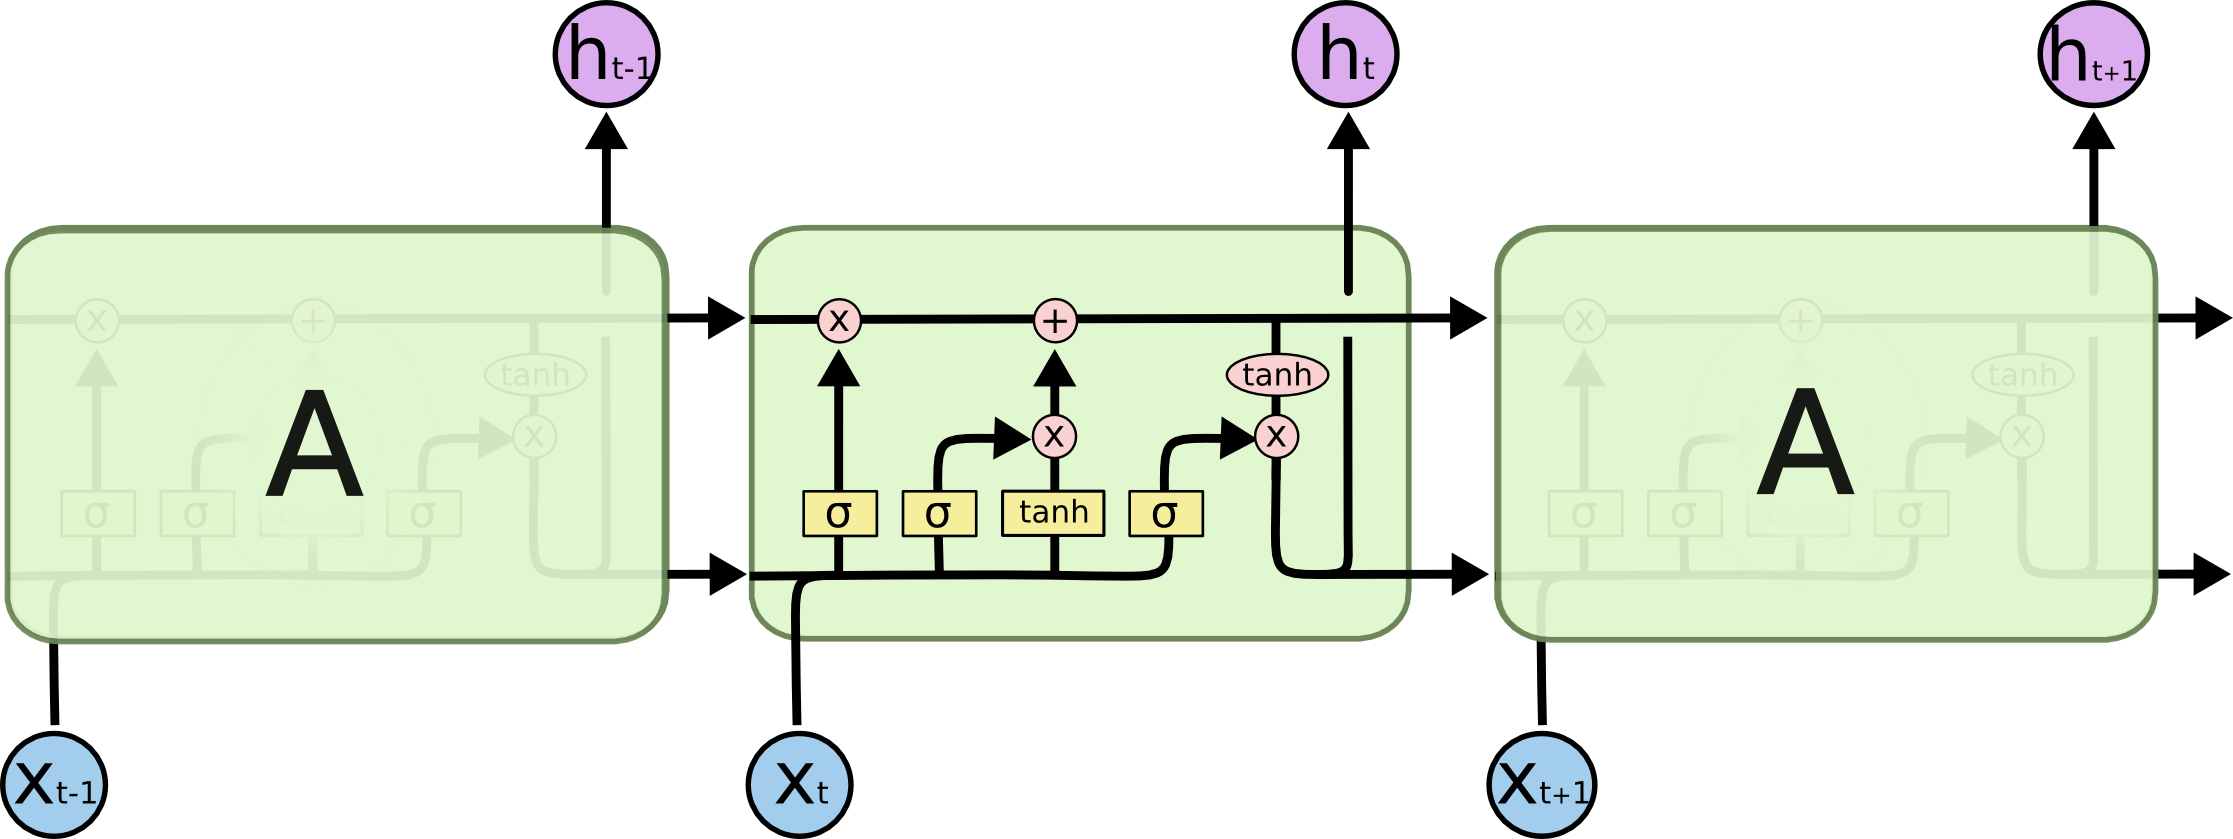
\includegraphics[scale=0.4]{monography/img/models/lstm3.png}
    \label{figure:lstm}
    \caption[Representação de uma arquitetura LSTM]{Representação de uma arquitetura LSTM\footnotemark}
\end{figure}
\footnotetext{\url{https://colah.github.io/posts/2015-08-Understanding-LSTMs/}}


Porém, diferentemente de uma \acrshort{RNN} comum, o LSTM possui uma camada a mais (além da \textit{Hidden Layer}) chamada de \textit{Cell State}. Esta camada é capaz de perceber as características mais latentes dos dados e descartar as menos importantes. Assim, o \acrshort{LSTM} consegue manter as características mais recorrentes na rede por mais tempo que uma \acrshort{RNN} comum. 

Na célula de memória do \textit{\acrshort{LSTM}}, existem estruturas que são responsáveis pela característica de memória a longo prazo e que são responsáveis por controlar a \textit{Cell State}. A Porta de Entrada, a Porta do esquecimento e a Porta de Saída. Abaixo está explicitado como cada um deles funciona:
%TODO: melhorar explicação das portas, principalmente a porta de saída 
%TODO: colocar fórmulas que explicam como o Ct é atualizado
\begin{itemize}
  \item Porta de Esquecimento: A primeira porta de uma célula do \acrfull{LSTM} decide qual informação provinda da célula anterior vai ser descartada. Isso é feito por meio de uma função de ativação sigmoidal que retorna um número entre 0 e 1 para cada valor da célula passada, onde 0 representa total esquecimento daquela informação e 1 total preservação.
  
  \item Porta do Entrada: A segunda porta decide qual informação deve ser atualizada. Para tal decisão são utilizadas duas funções. Primeiro, uma função sigmoid decide quais valores serão atualizados. Depois uma função Tahn cria novos valores candidatos a serem utilizados na atualização.
  \item Porta de Saída: Por fim, a porta de saída efetivamente faz as alterações nos valores da célula de memória atual. Os valores candidatos decididos na Porta de Entrada são colocados no lugar dos valores que devem ser atualizados.
\end{itemize}

% TODO: Falar que podemos responder a quantidade de camadas da LSTM com o problema que RNN tem com back-propagation que o gradiente começa a diminuir exponencialmente. Mas tem que dar uma conferida melhor.


\subsection{\acrfull{GRU}}

% TODO: da onde ta vindo essa explicação


%TODO: explicar diferenca entre porta da reinicializacao e porta da atualizacao, adicionando as fórmulas de cada uma

% TODO: falhas do GRU

\textit{\acrshort{GRU}} é um tipo de \textit{\acrshort{RNN}} semelhante ao \textit{\acrshort{LSTM}} e, assim como ele, também faz uso de mecanismos chamados de Portas que possibilitam que a informação seja atualizada ou esquecida ao ser transferida de uma célula para outra. Ou seja, \textit{\acrshort{GRU}} também é capaz de guardar informações importantes na rede de maneira mais eficaz que uma \textit{\acrshort{RNN}} comum. Apesar de parecidos, \textit{\acrshort{LSTM}} e \textit{\acrshort{GRU}} possuem algumas diferenças, como pode ser visto abaixo, o \textit{\acrshort{GRU}} possui apenas a \textit{Hidden Layer} e duas Portas para fazer o tratamento da informação para simular o efeito de memória:

\begin{itemize}
    \item Porta da atualização: A porta de atualização tem um papel semelhante às Portas de Entrada e Porta de Esquecimento do \textit{\acrshort{LSTM}}. Nela, é decidido quais dos valores provindos das células passadas serão adicionados a rede.
    \item Porta da reinicialização: Já o portão de reinicialização decide quanto da informação vinda das células passadas será esquecido.
\end{itemize}

Por ter uma arquitetura mais simples que uma \textit{\acrshort{LSTM}}, o \textit{\acrshort{GRU}} precisa de menos tempo para ser treinado e, geralmente, de menos dados também.

\begin{figure}[htbp]
    \centering
    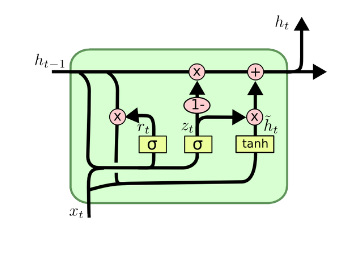
\includegraphics[scale=1.0]{monography/img/models/GRU.png}
    \label{figure:gru}
    \caption[Representação da arquitetura de uma GRU]{Representação da arquitetura de uma GRU\footnotemark}
\end{figure}